\documentclass[11pt]{article}
%==============================================================================
% Basic Packages {{{ 
%==============================================================================
\usepackage{mathpazo}
\usepackage[top=2cm, bottom=3.5cm, left=2.5cm, right=2.5cm]{geometry}

\usepackage{graphicx}                               %insert images
\usepackage{verbatim}                               %include txt files
\usepackage{cite}

\usepackage{amsmath,amsfonts,amssymb,amsthm}        %basic math support
\usepackage{tikz-cd}                                %draw commutative diagrams
\usetikzlibrary{graphs}                             %draw graphs with tikz
\usepackage{bussproofs}                             %proof trees
\usepackage{algorithm,algpseudocode}                %pseudocode algorithms

% }}}

%==============================================================================
% Page Setup {{{
%==============================================================================
\author{Eli Rosenthal \and Will Kochanski}
\date{}

\setlength{\parindent}{0pt}
% }}}

%==============================================================================
% Macros {{{
%==============================================================================
\newcommand{\img}[1]{\begin{center}
    \includegraphics[width=0.8\textwidth]{#1}
\end{center}}

\newenvironment{bprooftree}
    {\leavevmode\hbox\bgroup}
    {\DisplayProof\egroup}

\newcommand{\ir}[1]{\textnormal{\sc#1}}
\newcommand{\tx}[1]{\textnormal{#1}}
\newcommand{\arr}{\rightarrow}

\newcommand{\R}{\mathbb{R}}


\newtheorem{Thm}{Theorem}
\newtheorem{Lem}{Lemma}
\newtheorem{Cor}{Corollary}
% }}}

\title{Paper Summary: Probabilistic Encryption}
\begin{document}
%==============================================================================
% Begin Document
%==============================================================================
\maketitle
\section{Introduction}
In the paper ``An Elementary Proof of a Theorem of Johnson and
Lindenstrauss''~\cite{mainpaper}  Dasgupta and Gupta reprove a major
dimensionality reduction result of Johnson and Lindenstrauss in~\cite{oldpaper}.
Their approach is interesting for the simplicity of its presentation and use of
relatively elementary probabilistic techniques.

\section{Dimensionality Reduction}
In data analysis we often want to produce summary information to describe a large data set. A natural extension of this is to ask whether we can find a smaller repesentation of our data which preserves the overall structure. In many cases our data can be represented as a set of points, $V$, in some high dimensional euclidean space, $\R^d$. In this setting we ask whether there is a linear map
\[ f : \R^d \arr \R^k \]
To some lower dimensional space without distorting the data too much. Intuitively we can think of this as choosing $k$ features to represent our data, and discarding everything else. For example the data set visualized here

\section{Dimensionality Reduction}
In data analysis we often want to produce summary information to describe a
large data set. A natural extension of this is to ask whether we can find a
smaller repesentation of our data which preserves the overall structure. In many
cases our data can be represented as a set of points, $V$ in some high
dimensional euclidean space $\R^d$.
>>>>>>> updated spheres, modified writeup format

\begin{center}
    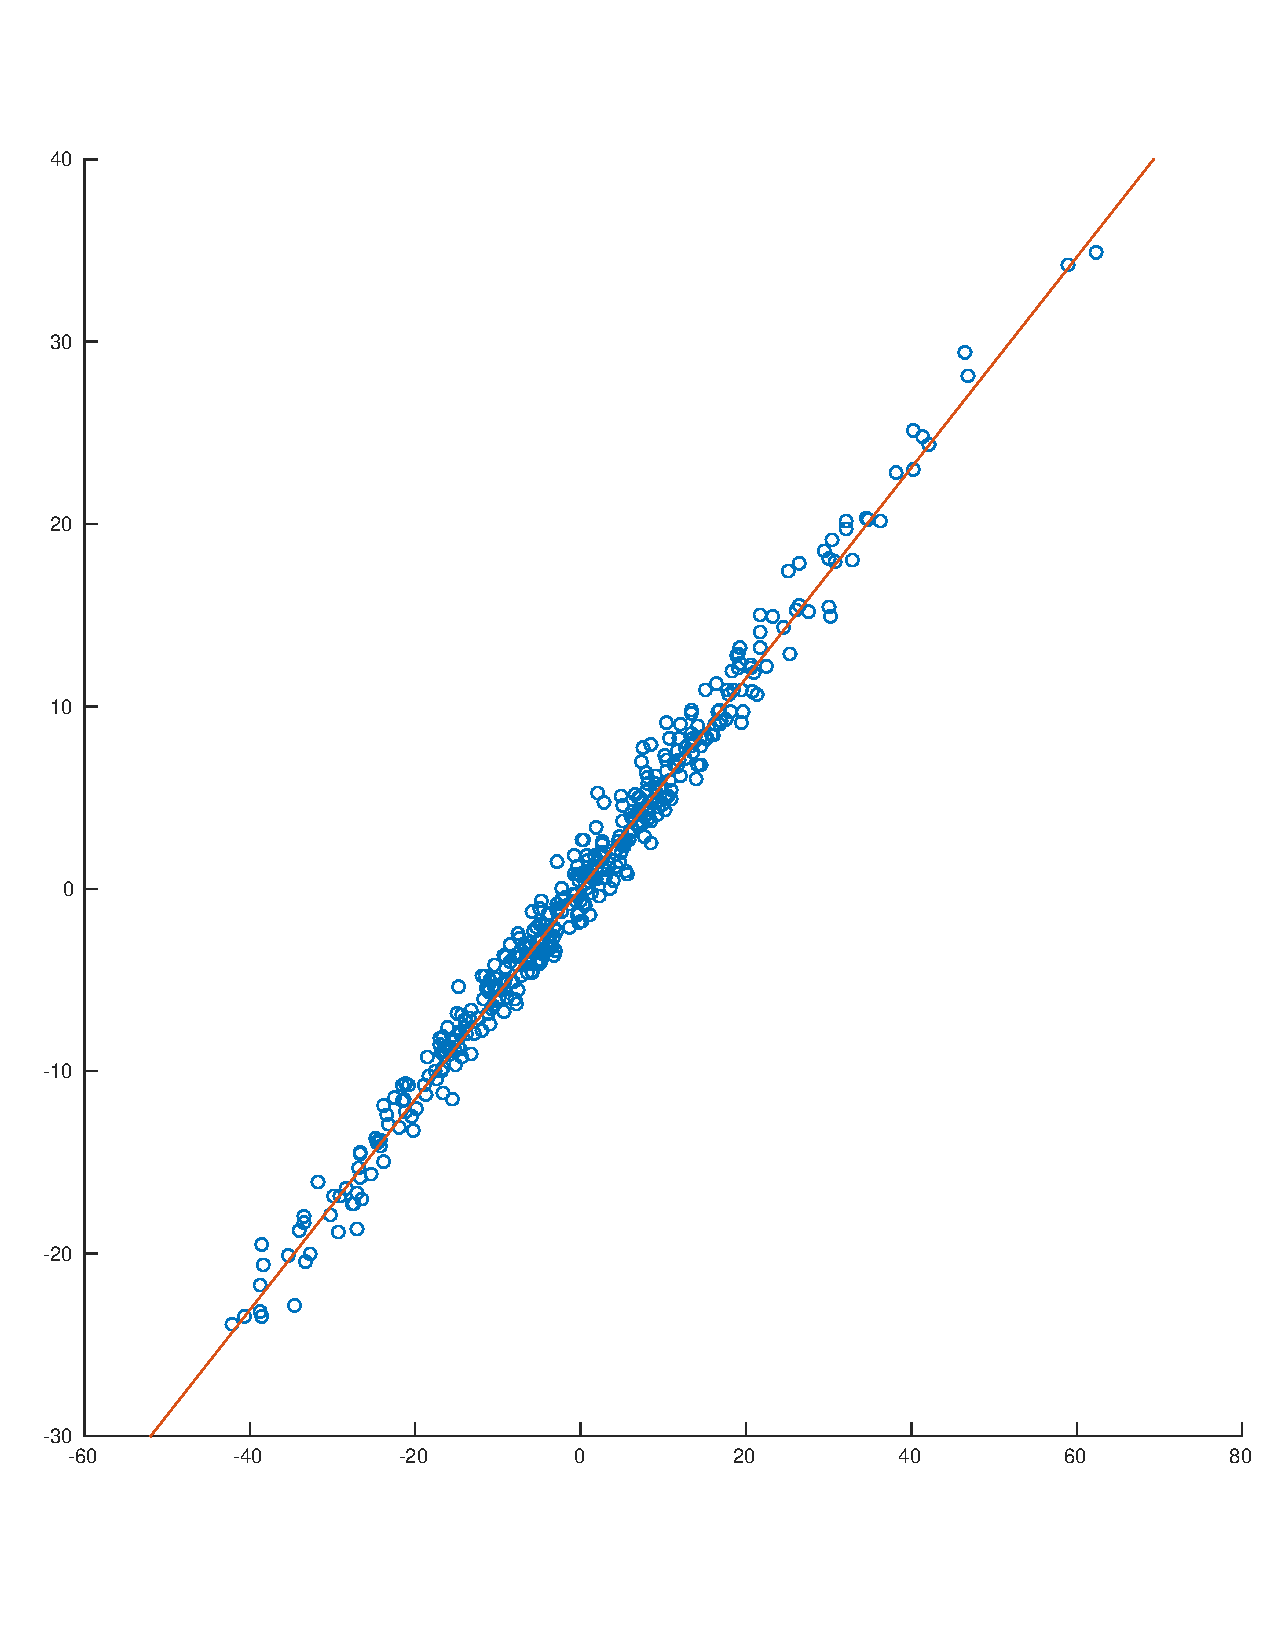
\includegraphics[trim=0 240 0 280, clip,width=0.7\textwidth]{2dprimaryaxis.pdf}
\end{center}

Can be represented almost faithfully by projecting onto the one dimensional space represented by the central line. The surprising result of Johnson and Lindenstrauss is that in high enough dimensions we can choose a \textit{random} projection without distorting the data too much.


\section{The Johnson Lindenstrauss Theorem}
\begin{Thm}

    For any $0 \leq \epsilon \leq 1$, and any integer $n$, let $k$ be a positive
    integer such that
    \[ 
      k \geq 4(\epsilon^2/2 - \epsilon^3/3)^{-1} \ln n 
    \]
    Then for any set of $n$ points $V \subseteq \R^d$, there exists a map
    $f:\R^d \arr R^k$ such that for all $u, v \in V$
    \[
      (1-\epsilon)\|u - v\|^2 \leq \| f(u) - f(v) \|^2 \leq (1+\epsilon) \| u - v \|^2 
    \]
    Furthermore, this map can be found in randomized polynomial time.
\end{Thm}

-- Statement of the theorem
-- Contextualization of variables
-- Intution, when projected length is tightly concentrated around mean

-- Intuition for a random projection
-- rotational invariance, linear scaling, allows us to analyse a random vector.

\subsection{Sampling from the Unit Sphere}
-- Why it might be difficult
-- first attempt using polar coordinates

-- Key realization: We can impose constraints *after* sampling
   -- all we need is a rotationally symmetric distribution
-- Enter gaussians, why do they work.
-- Other key advantage: Now each component is i.i.d
    -- Makes projection very easy to reason about.

\section{Large Deviation Bounds}
-- Remains to analyse the result of the projetion
-- Probabilistic method, low failure for each distance, take union bound, repeat until success to get
-- randomized algorithms

??? how much detail into math do we want to give?


\section{Comparison to other Approaches}
-- what kinds of properties we might be interested in preserving
-- the role of randomness (i.e. avoiding selecting features, ease of use, streaming computation)


\section{Initial notes}

Dimensionality reduction is an important 
- why we care about DR
- in particular, this version is pretty cool

- rotational invariance of the joint distribution, 
- how do we go about vvv 
- sampling from a smooth surface
- are gaussians always the answer?
showing why the gaussian stuff is rotationally invariant
- talking about chernoff bounds
\bibliography{refs}{}
\bibliographystyle{plain}

\end{document}
